\documentclass[a4paper,10pt]{article}
\usepackage[utf8]{inputenc}
\usepackage{graphicx}
\usepackage{caption}
\usepackage{subcaption}
\usepackage[left=1.0in, right=1.0in]{geometry}
\usepackage[section]{placeins}

%opening
\title{Multiblock Data Parallel Surface LIC}
\author{Burlen Loring}

\begin{document}

\maketitle

\begin{abstract}

\end{abstract}

\section{Features for interactive data exploration}
\subsection{Pipeline}

\begin{figure}[ht]
	\centering
	\begin{subfigure}{0.55\textwidth}
		\centering
		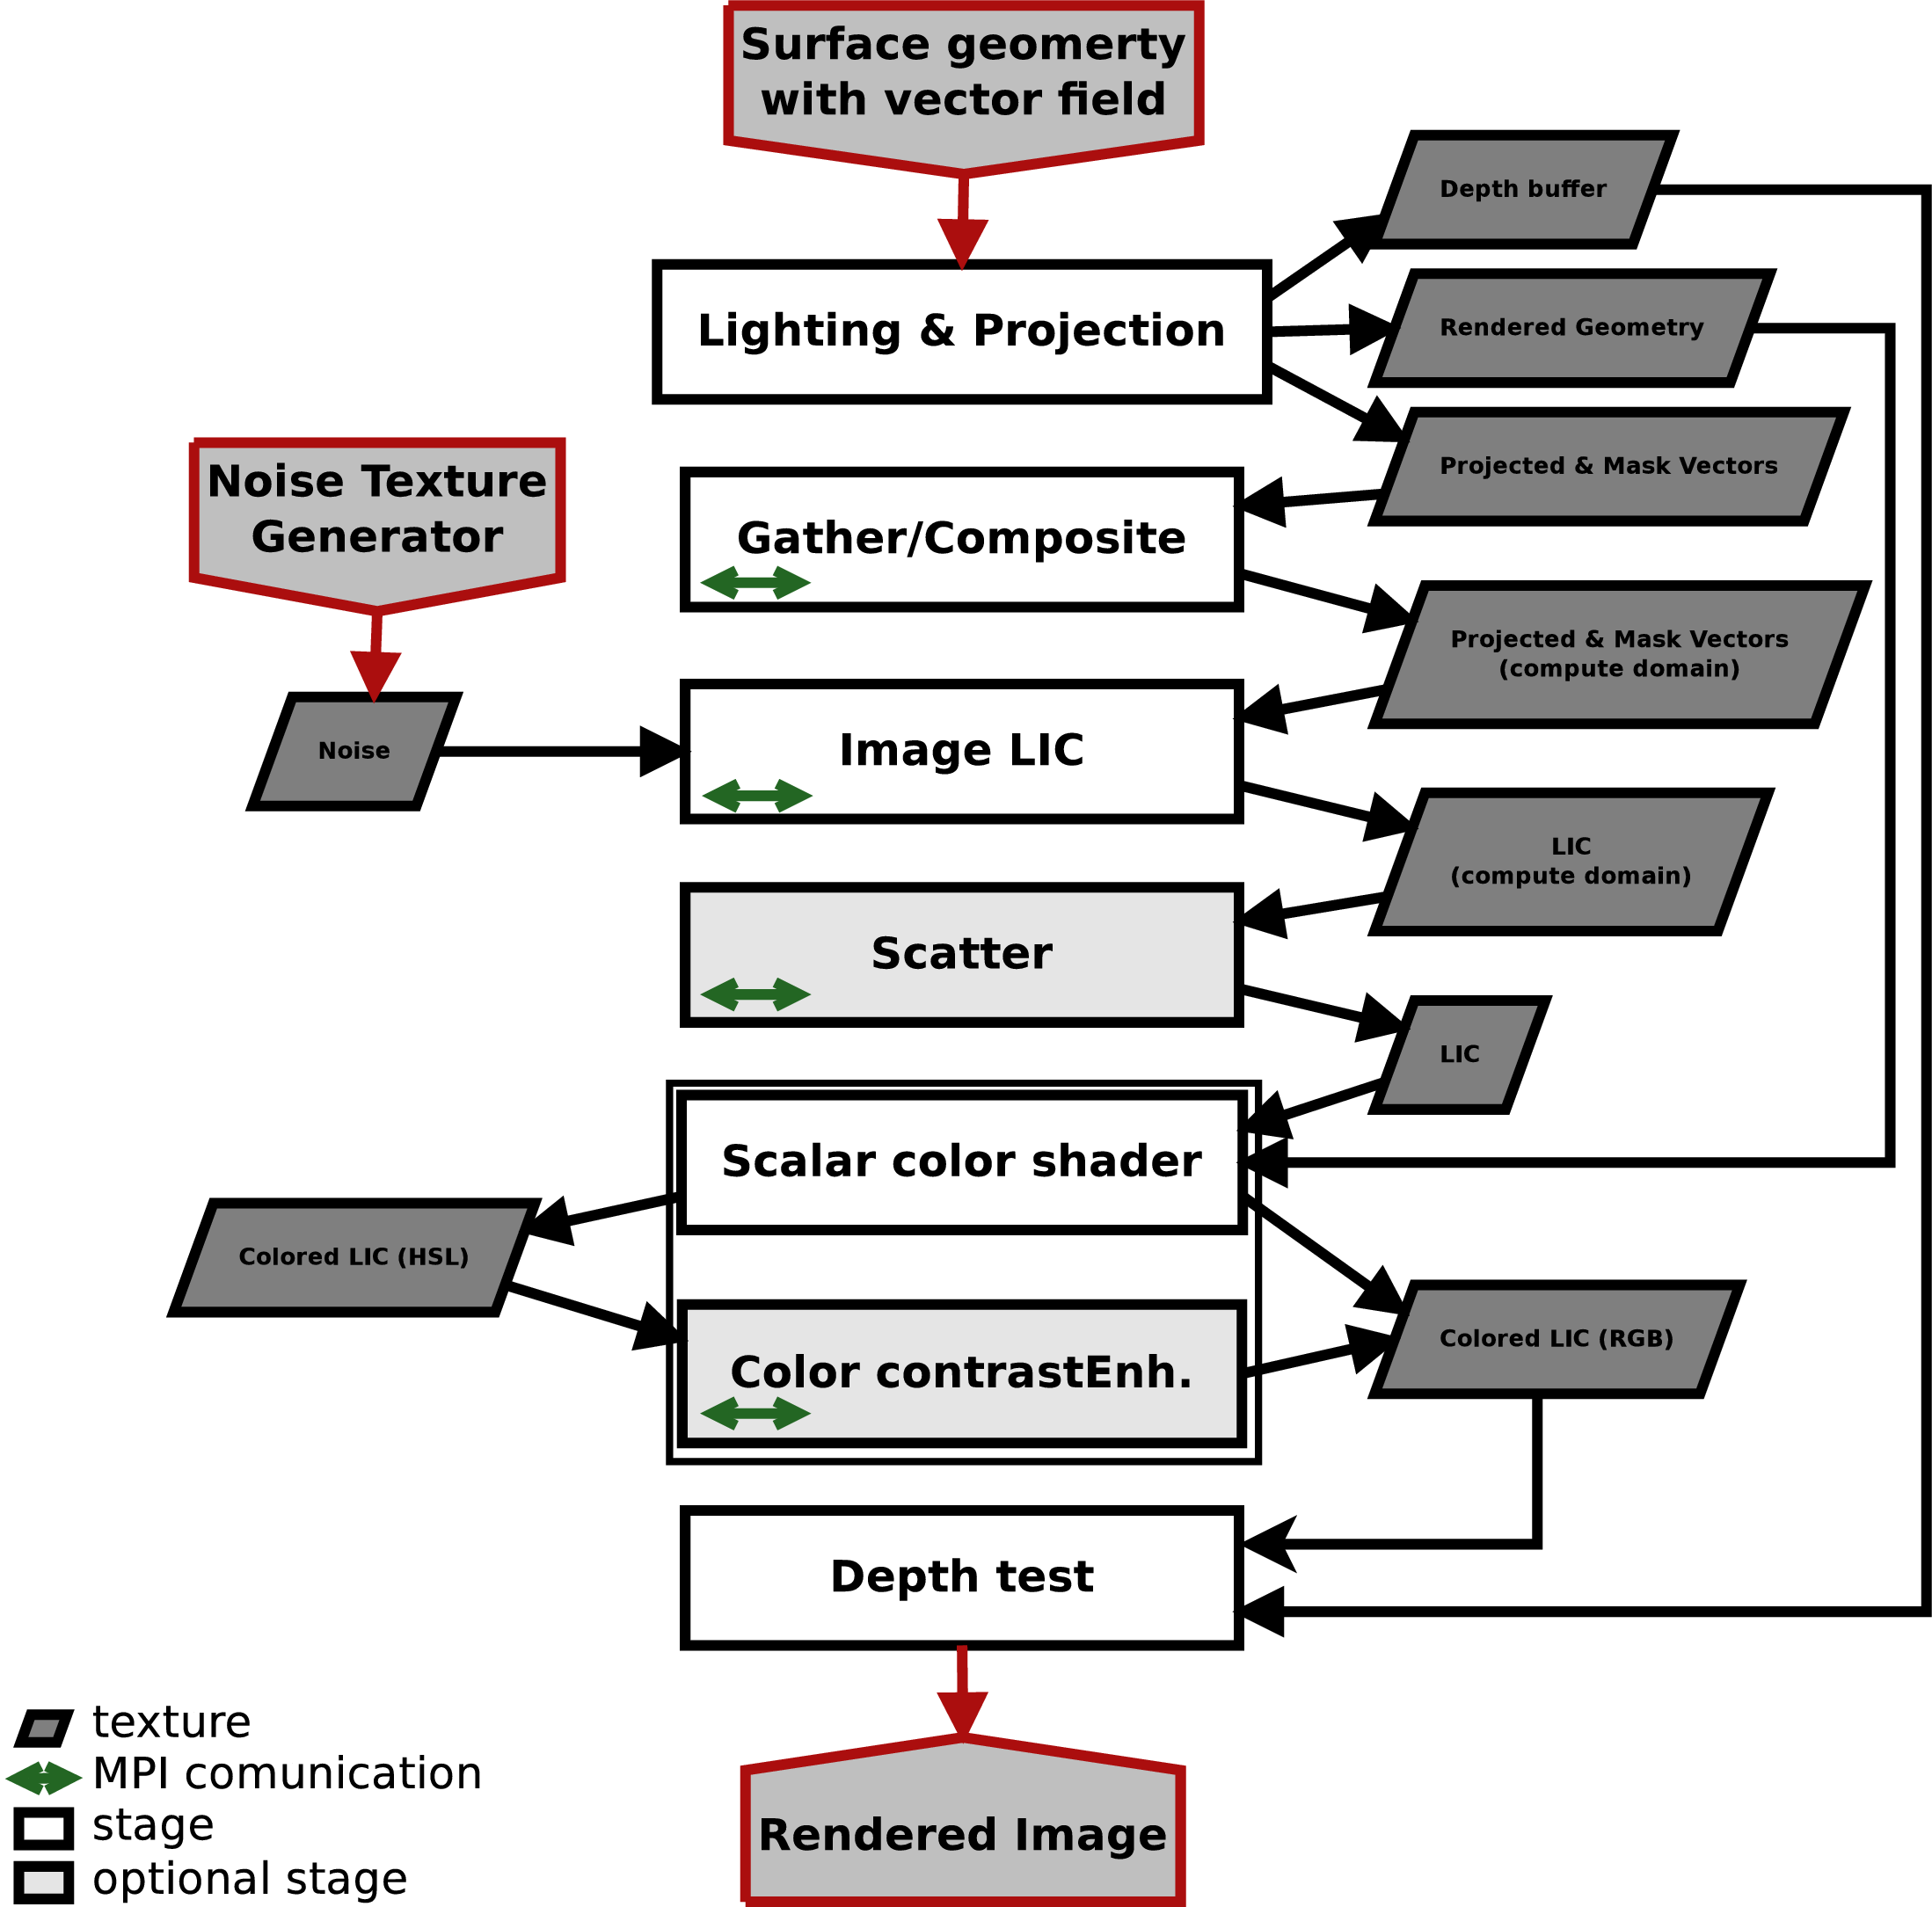
\includegraphics[width=\textwidth]{./images-data/dia-serial/surfacelic-painter-flow.png}
		\caption{}
		\label{fig:lic2d-flow}
	\end{subfigure}
% 	\hspace{0.1in}
	\begin{subfigure}{0.4\textwidth}
		\centering
		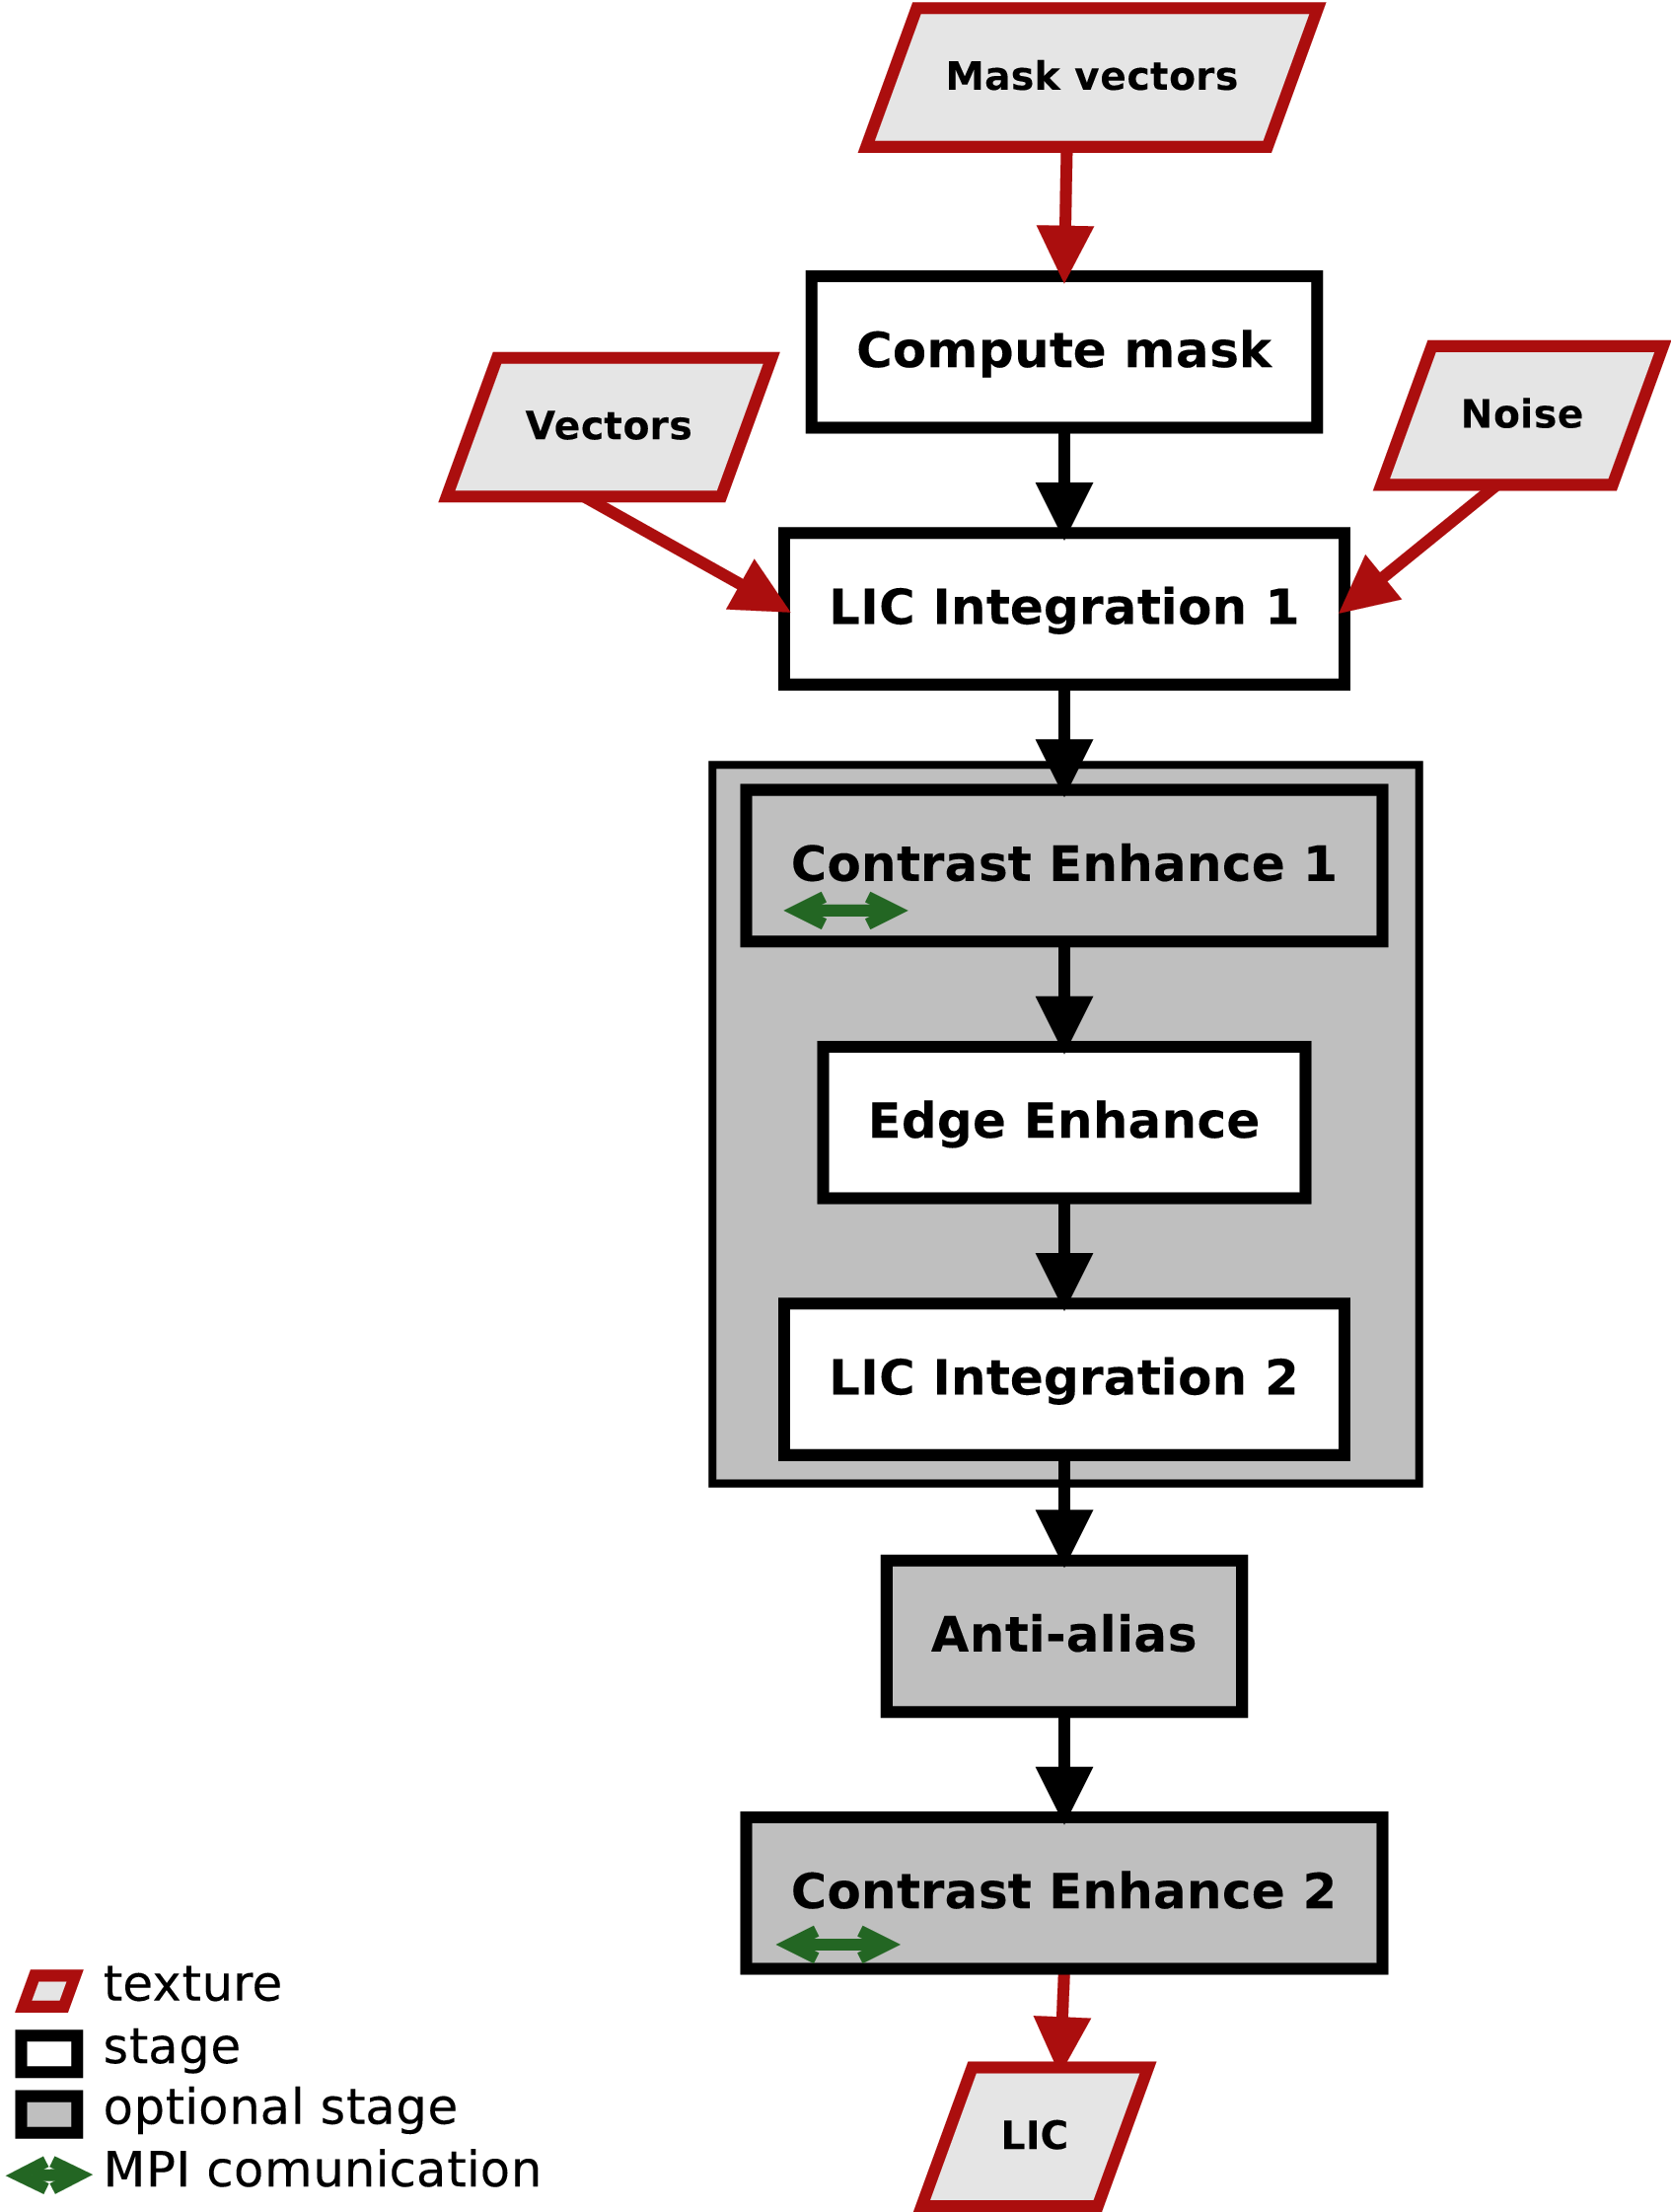
\includegraphics[width=\textwidth]{./images-data/dia-serial/lic2d-flow.png}
			% lic2d-flow.eps: 0x0 pixel, 300dpi, 0.00x0.00 cm, bb=0 0 610 807
		\caption{}
		\label{fig:lic2d-flow}
	\end{subfigure}
\end{figure}

\begin{figure}[ht]
	\centering
	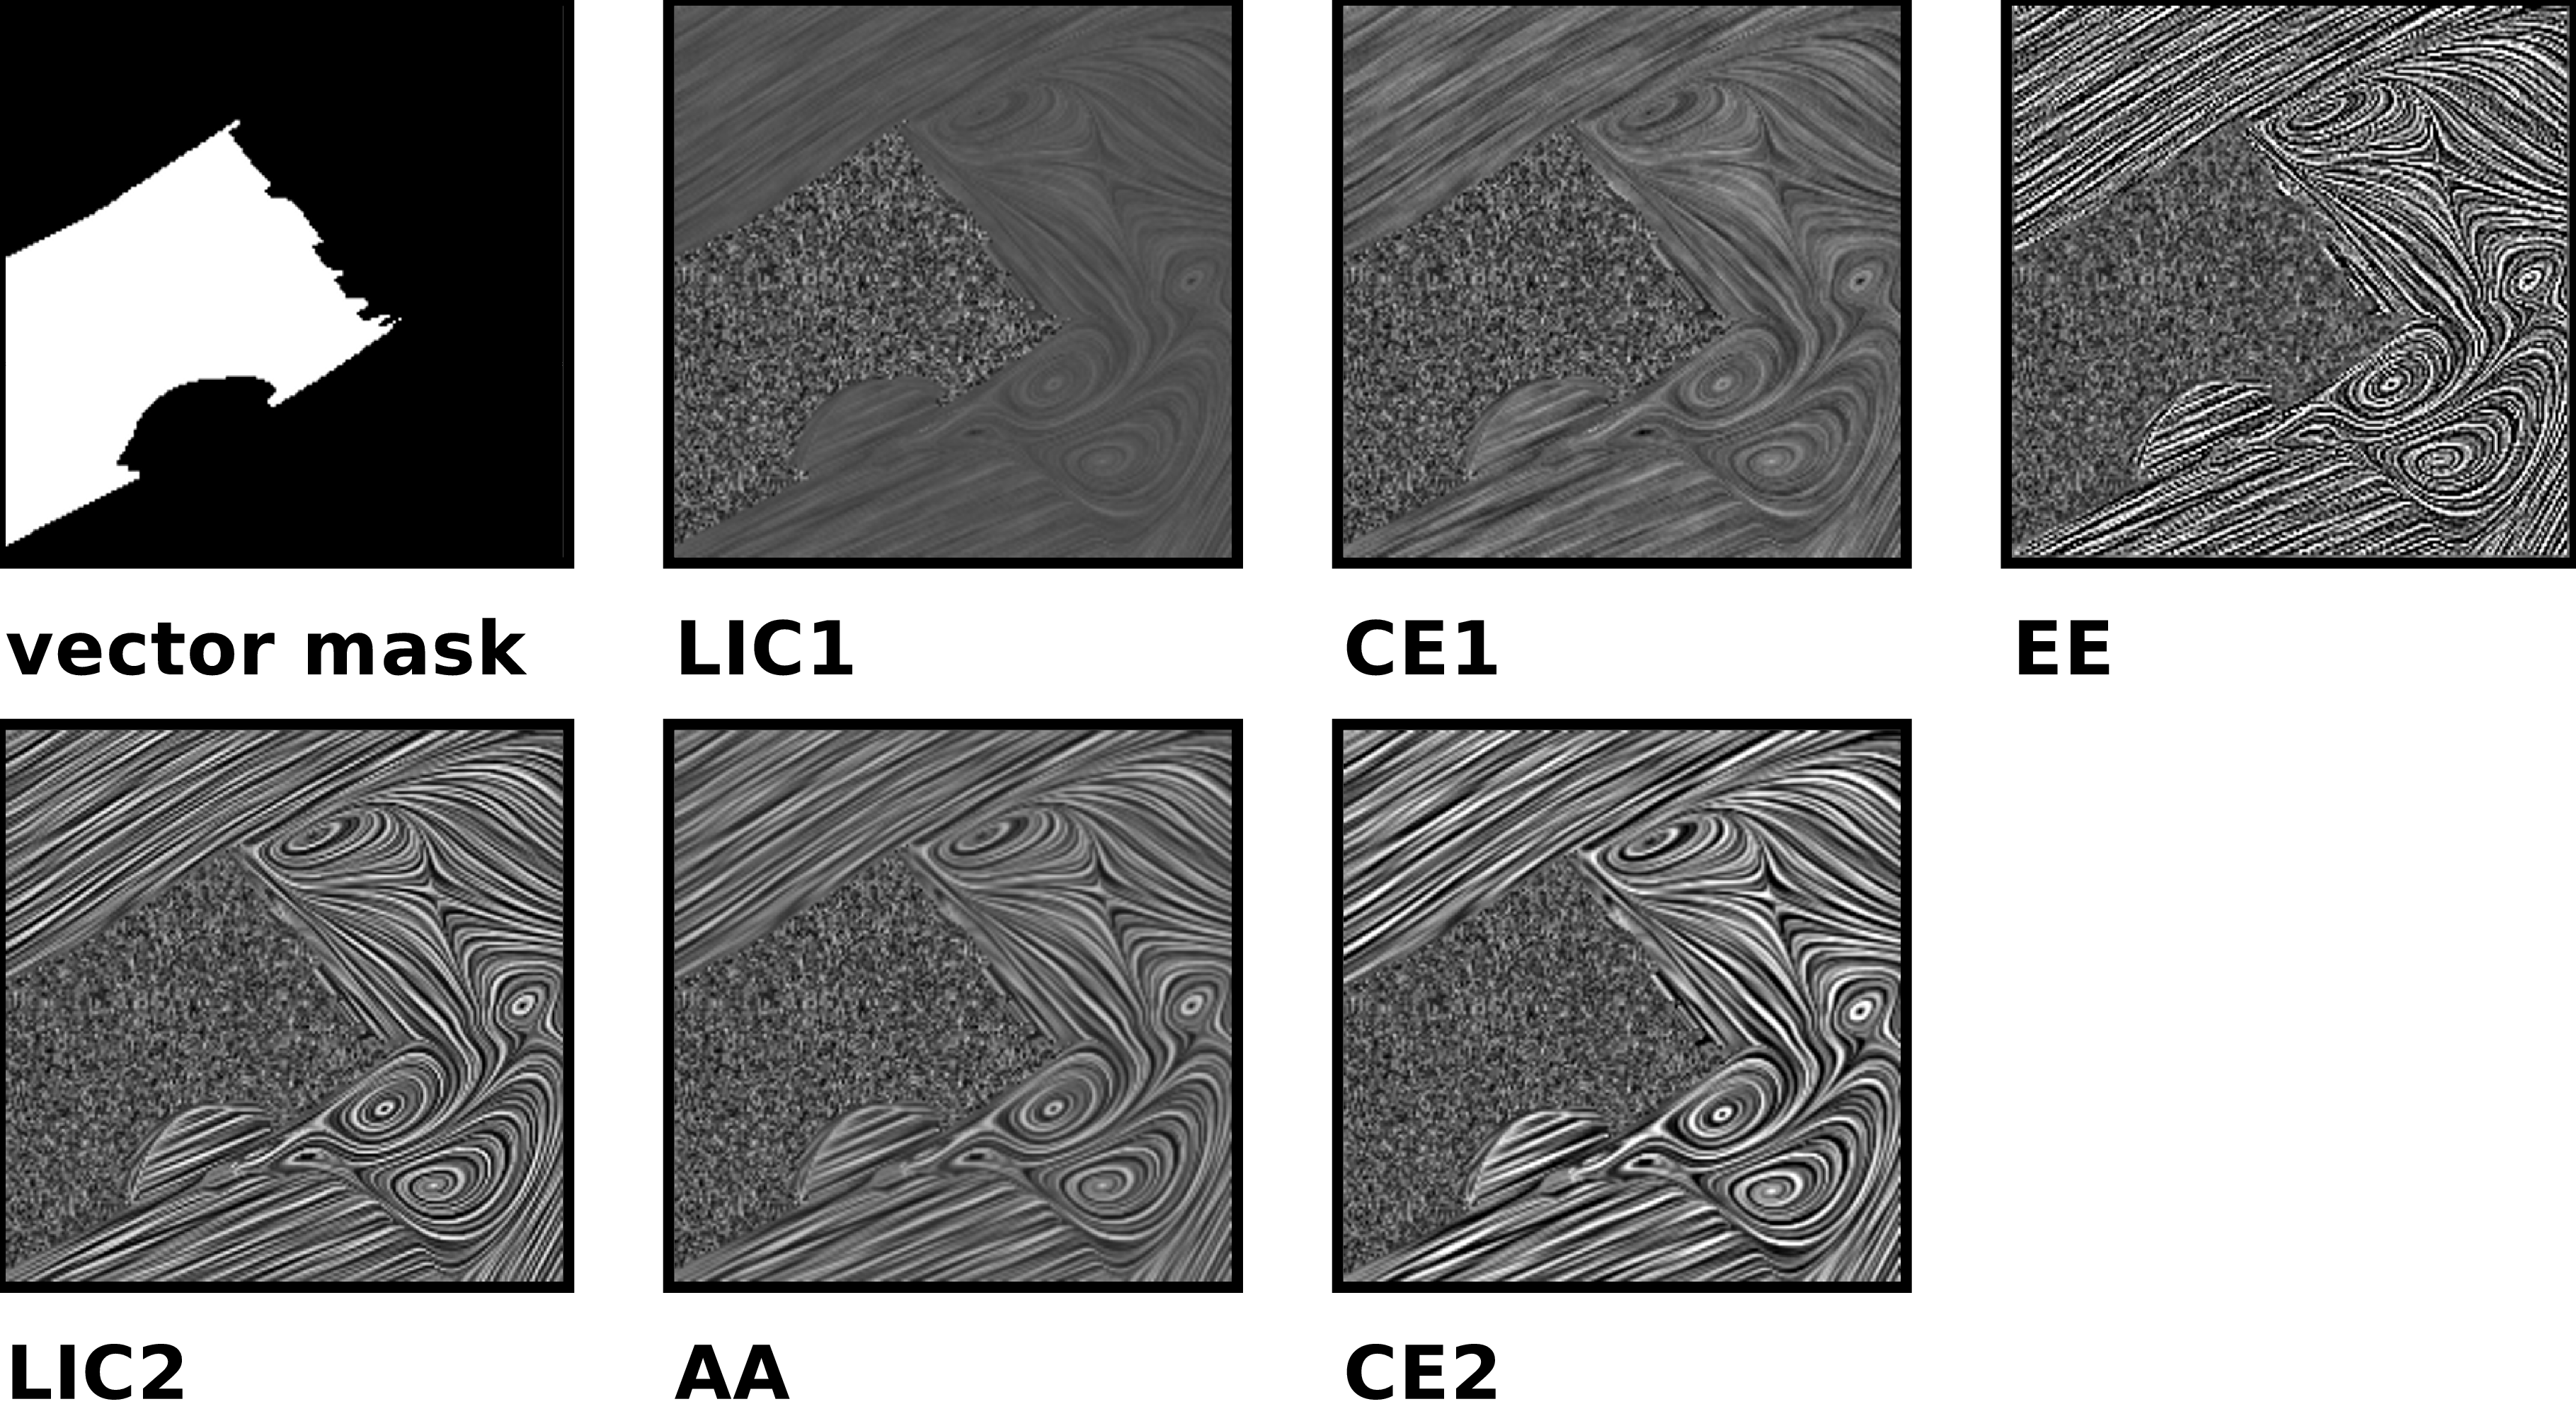
\includegraphics[width=0.75\textwidth]{./images-data/dia-serial/lg-lic2d-200ppi.png}
	% lic2d-flow.eps: 0x0 pixel, 300dpi, 0.00x0.00 cm, bb=0 0 610 807
	\label{fig:lic2d-outputs}
  \caption{Line integral 2D stages}
\end{figure}

\begin{figure}[ht]
	\centering
	\includegraphics[width=0.75\textwidth]{./images-data/dia-serial/lg-surface-lic-painter-200ppi.png}
	\label{fig:lic2d-outputs}
  \caption{Surface LIC Painter stages}
\end{figure}

% \subsection{vtkSurfaceLICPainter}
The pipeline employed by the vtkSurfaceLICPainter, including the new contrast enhancement stages, is shown in the following schematic:
\begin{center}
\footnotesize\bf
\begin{verbatim}
         noise
           |
           [ PROJ LIC2D COLOR (CCE) ]
           |                        |
        vectors                  surface LIC
\end{verbatim}%
\end{center}
Where, the PROJ stage renders geometry, projecting vectors onto the surface, and the the screen; the LIC2D stage computes the LIC driving the vtkLineIntegralConvolution2D class; the COLOR stage combines LIC with scalar colors shading the surface geometry; and the CCE stage applies the new color contrast enhancement. Optional stages are enclosed in ().

In order to provide better interaction and faster response as parameters are varied during interactive exploration, each stage renders to a frame-buffer which is cached. This enables un-necessary stages to be skipped during interaction. For example, if an integrator parameter is modified then the geometry rendering and projection stage can be skipped. For large data this optimization can result in orders of magnitude speed up during interaction.

% \subsection{vtkLineIntegralConvolution2D}
The pipeline employed in vtkLineIntegralConvolution2D, including the new contrast enhancement stages, is shown in the following schematic:
\begin{center}
\footnotesize\bf
\begin{verbatim}
  noise texture
           |
           [ LIC ( ( CE ) HPF LIC ) ( AA ) ( CE ) ]
           |                                      |
  vector texture                              LIC'd image
\end{verbatim}%
\end{center}
Where LIC is the line integral convolution stage, HPF is a high-pass filter stage, CE is a contrast enhancement stage, and AA is an anti-aliasing stage. The optional stages are enclosed in (). Nested optional stages depend on the execution of their parent stage.

\FloatBarrier

\subsection{Noise generator}
The streak characteristics and look of the final LIC'ed image vary widely based on the input dataset, resolution of the final image, and choice of surface geometry. One important factor in determining the streaking characteristics and overall look of the final image are the characteristics of the input noise texture. The size of the noise pixels, the size of the noise texture, the contrast and dynamic range of the noise texture, all play a role in the look of the final image. Using the same noise texture produces markedly different results on different datasets and even on the same dataset at different screen resolutions. It's unlikely that a single noise texture will work well in all cases.

In order to provide more control over the streaking characteristics and general look of the final LIC image I have added customizable noise texture generator. The noise texture can be modified based on the following parameters:

\begin{description}
\item[GenerateNoiseTexture] Select between the default static noise texture or generate a custom noise texture using the following parameters.
\item[NoiseType] Select between Gaussian, uniformly distributed noise, or Perlin noise.
\item[NoiseTextureSize] Select the number of pixels in a side of the square noise texture.
\item[NoiseGrainSize] Select the number of pixels each side of the square noise value spans.
\item[MinNoiseValue] Set the lowest color in the noise texture, the default, 0, is black.
\item[MaxNoisevalue] Set the highest color in the noise texture, the default, 1, is white.
\item[NumberOfNoiseLevels] Set the number of noise colors.
\item[ImpulseNoiseProbability] Impulse noise noise can be generated with a probability less than 1.
\item[ImpulseNoiseBackgroundColor] The color to use for un-touched pixels.
\item[NoiseGeneratorSeed] Modify the seed value of the random number generators.
\end{description}

Changing the noise texture gives one greater control over the look of the final image. By default the original static 200x200 noise texture (see VTKData/Data/Data/noise.png) is used.

\subsection{Scalar color shading}
The current approach for shading the LIC'ed image with scalar colors blends the scalar colors with the LIC according to
\begin{equation}
c_{ij} = L_{ij} * I + S_{ij} * (1 - I)
\label{eqn:color-blend}
\end{equation}
where the indices $i,j$ identify a specific fragment, $c$ is final RGB color, $L$ is LIC gray scale value, $S$ is the scalar RGB color, and $I$ is a constant ranging from 0 to 1, with a default of 0.8. Decreasing $I$ to obtain brighter colors diminishes the intensity of the LIC, and vise versa. When colors are bright the LIC is difficult to see. Currently, the best results are obtained by sacrificing on both fronts.

The purpose of the new scalar color shader is to provide both bright and intense scalar colors without diminishing the visibility of the LIC itself. The shader is implemented by the following equation:
\begin{equation}
c_{ij} = ( L_{ij} + f ) * S_{ij}
\label{eqn:color-map}
\end{equation}
where the indices $i,j$ identify a specific fragment, $c$ is final RGB color, $L$ is LIC gray scale intensity, $S$ is the scalar RGB color, and $f$ is a biasing parameter, typically 0, that may be used for fine tuning. When $f=0$, the typical case, colors are transfered directly to the final image where the LIC is 1, and a linearly scaled transfer of scalar colors where LIC gray scale color is less than one down to 0, where the final color is black. The bias parameter $f$ may be set to small positiver or negative values between -1 and 1 to increase or decrease LIC values uniformly resulting in brighter or darker images. When $f\neq0$ final fragment colors, $c$, are clamped such that $0 \leq c \leq 1$.

\subsection{Contrast enahancement}

\begin{figure}[ht]
 \centering
\begin{subfigure}{0.48\textwidth}
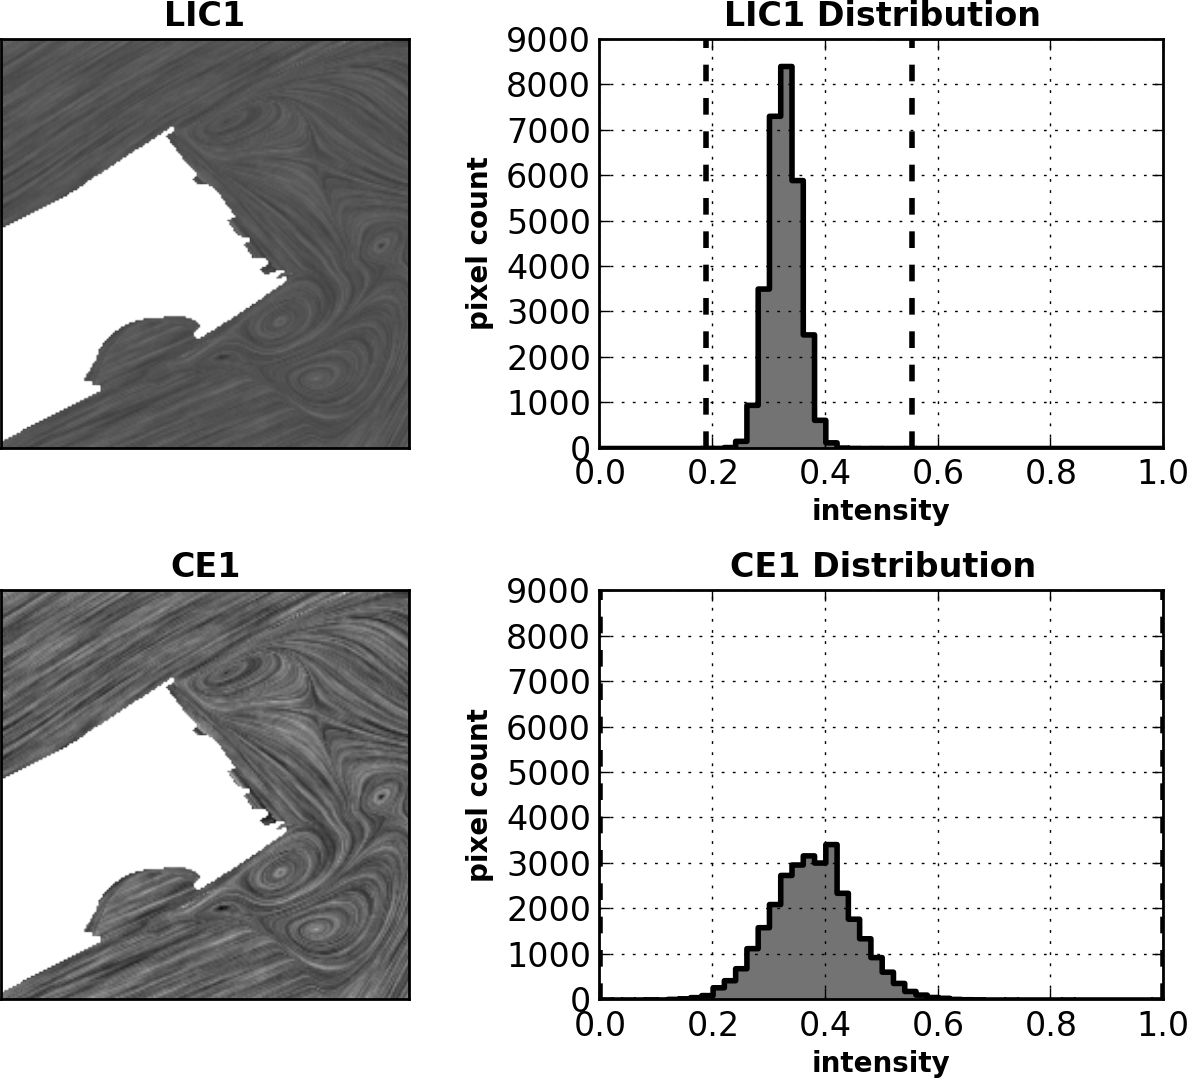
\includegraphics[width=\textwidth]{./images-data/dia-serial/gray-ce1-curves.png}
% gray-ce1-curves.png: 1187x1078 pixel, 200dpi, 15.07x13.69 cm, bb=0 0 427 388
\caption{}
\label{fig:gray-ce-curves1}
\end{subfigure}
\hspace{0.15in}
\begin{subfigure}{0.48\textwidth}
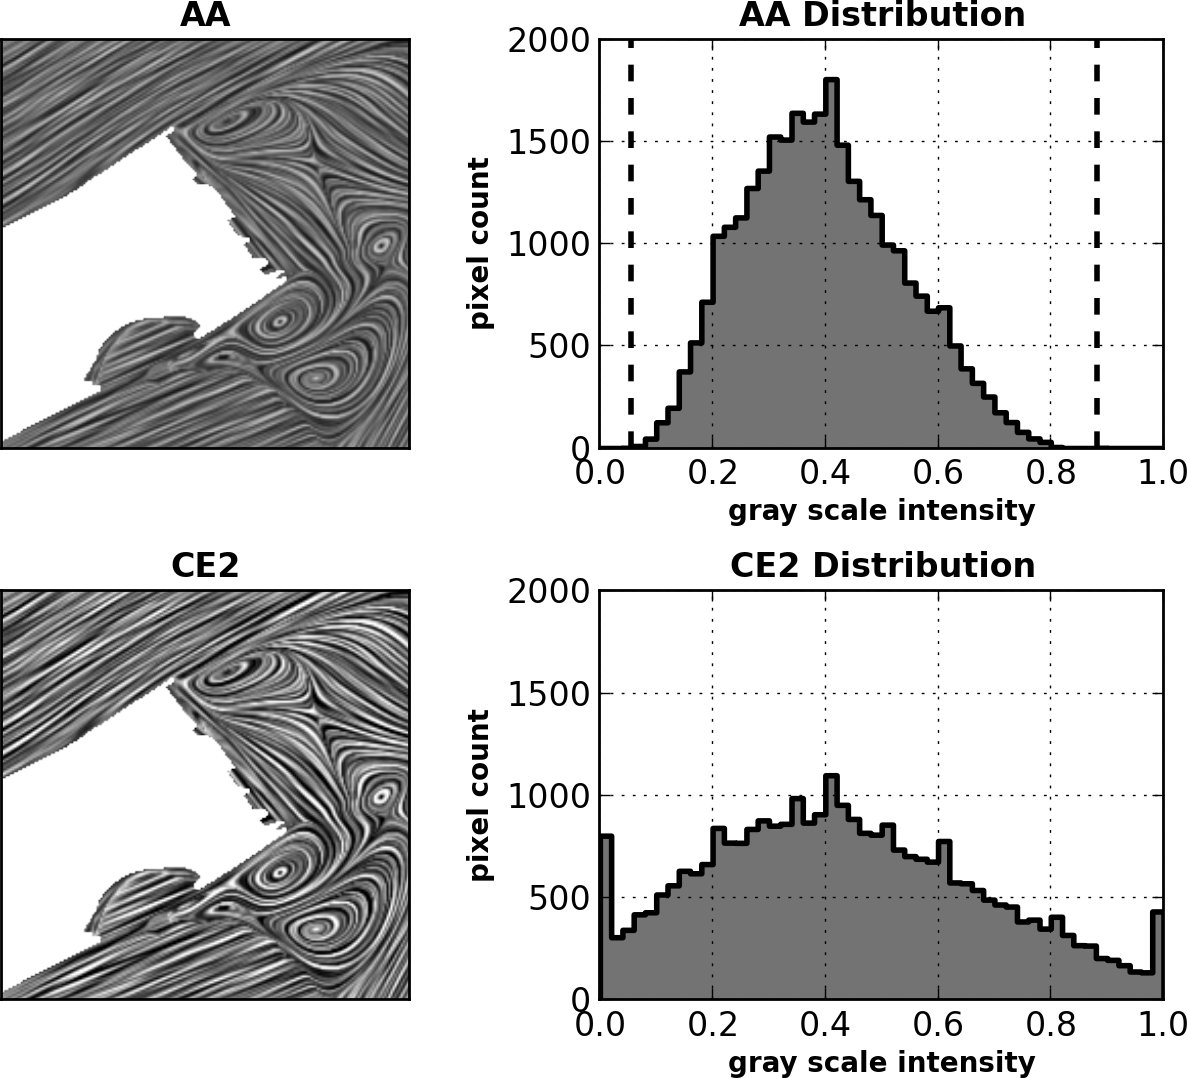
\includegraphics[width=\textwidth]{./images-data/dia-serial/gray-ce2-curves.png}
% gray-ce1-curves.png: 1187x1078 pixel, 200dpi, 15.07x13.69 cm, bb=0 0 427 388
\caption{}
\label{fig:gray-ce-curves2}
\end{subfigure}
\end{figure}

\label{sec:contrast}
The convolution process tends to decrease both contrast and dynamic range, often producing dark and dull results. Figure \ref{fig:motivation}.a illustrates this issue. The narrowing of dynamic range and diminishing of contrast are consequences of the convolution operation which convolves a noise texture with a vector field. These reductions are made worse by the use of  Gaussian noise because by definition centrally concentrates its values about a mid gray tone.

In order to counteract this, optional contrast enhancement stages have been added. The new stages increase the dynamic range and contrast without modifying the patterns that emerge from the LIC process or modifying the scalar colors. VTK's surface LIC implementation is provided by two classes, the vtkSurfaceLICPainter and vtkLineIntegralConvolution2D. The vtkSurfaceLICPainter, projects vectors, sets up noise texture, and passes control to the vtkLineIntegralConvolution2D to generate a LIC, after which it shades scalar colors combined with the generated LIC onto the surface geometry. Contrast enhancement stages have been added to both classes.


% \subsection{vtkLineIntegralConvolution2D}
The contrast enhancement stages are implemented by histogram stretching of the gray scale colors in the LIC'ed image as follows:
\begin{equation}
c_{ij} = \frac{c_{ij} - m}{M - m}
\end{equation}
where, the indices $i,j$ identify a specific fragment, $c$ is the fragment's gray scale color, $m$ is the gray scale color value to map to 0, $M$ is the gray scale color value to map to 1. When the contrast enhancement stage is applied on the input of the high-pass filter stage, $m$ and $M$ are always set to the minimum and maximum gray scale color of all fragments. In the final contrast enhancement stage $m$ and $M$ take on minimum and maximum gray scale colors by default but may be individually adjusted by the following set of equations:
\begin{equation}
m = min(C) + F_{m} * ( max(C) - min(C) )
\end{equation}
\begin{equation}
M = max(C) - F_{M} * ( max(C) - min(C) ) 
\end{equation}
where, $C = \{c_{00},c_{01},...,c_{nm}\}$, are all of the gray scale fragments in the LIC image and $F_m$ and $F_M$ are adjustment factors that take on values between 0 and 1. When $F_m$ and $F_M$ are 0 minimum and maximum are gray scale values are used. This is the default. Adjusting $F_m$ and $F_M$ above zero controls the saturation of normalization. This is useful, for example, if the brightness of pixels near the border dominate because these are convolved less because we can't integrate outside of the dataset.

Occasionally, often depending on the contrast and dynamic range and graininess of the noise texture, jagged or pixelated patterns may emerge in the LIC. These can be reduced by enabling the optional anti-aliasing pass.


\begin{figure}[ht]
\centering
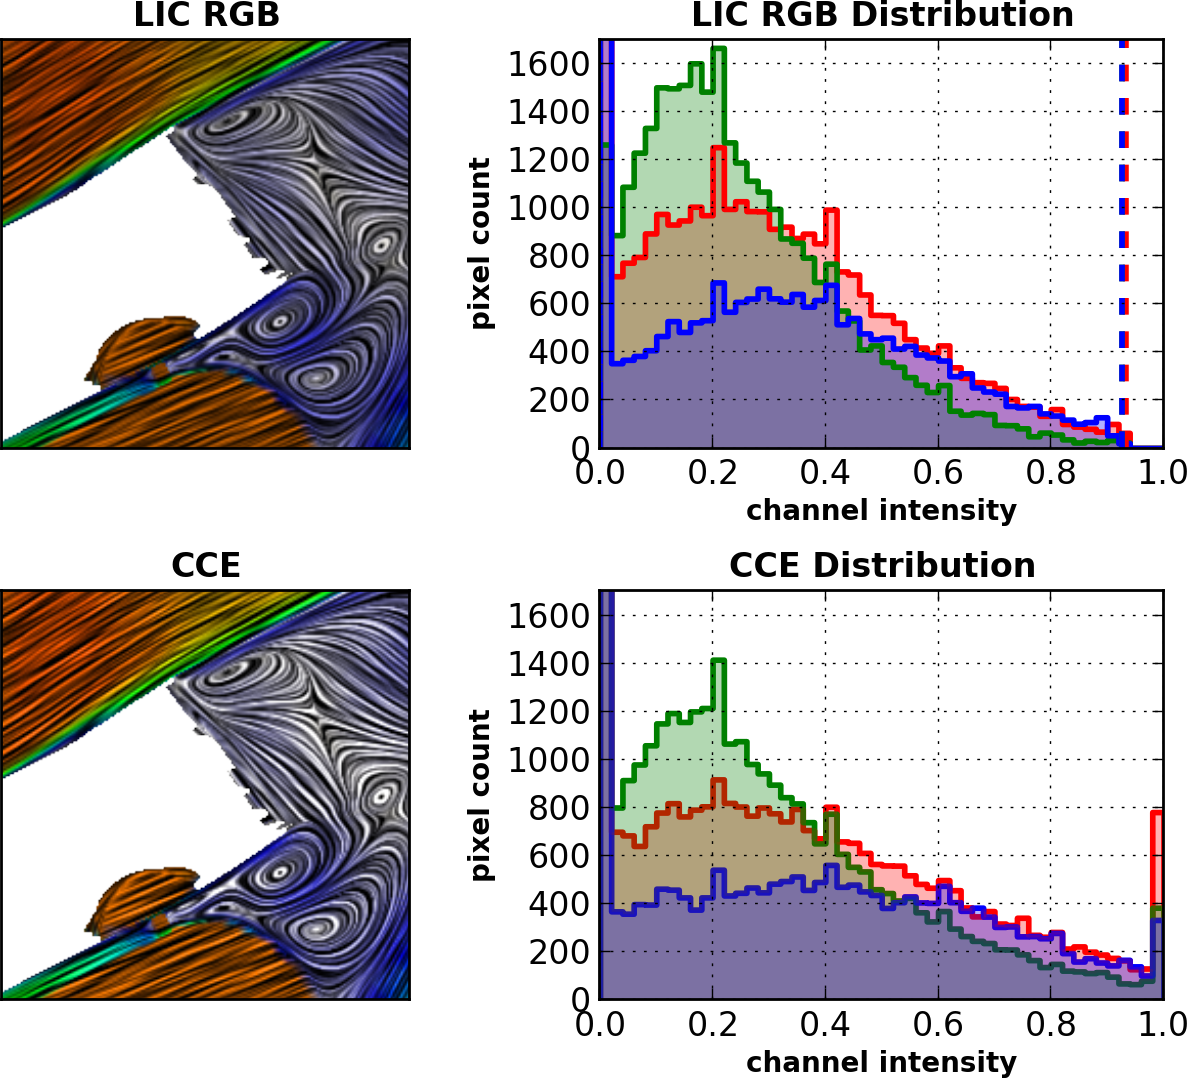
\includegraphics[width=0.48\textwidth]{./images-data/dia-serial/color-ce-curves.png}
% gray-ce1-curves.png: 1187x1078 pixel, 200dpi, 15.07x13.69 cm, bb=0 0 427 388
\caption{CE Curves}
\label{fig:gray-ce-curves2}
\end{figure}
% \subsection{vtkSurfaceLICPainter}
The color contrast enhancement stage is implemented with histogram stretching on the fragments lightness in the HSL color space.
\begin{equation}
L_{ij} = \frac{L_{ij} - m}{M - m}
\end{equation}
where, the indices $i,j$ identify a specific fragment, $L$ is the fragment's lightness in HSL space, $m$ is the lightness to map to 0, $M$ is the lightness to map to 1. $m$ and $M$ take on minimum and maximum lightness over all fragments by default but may be individually adjusted by the following set of equations:
\begin{equation}
m = min(L) + F_{m} * ( max(L) - min(L) )
\end{equation}
\begin{equation}
M = max(L) - F_{M} * ( max(L) - min(L) ) 
\end{equation}
where, $L$ are fragment lightness values and $F_m$ and $F_M$ are the adjustment factors that take on values between 0 and 1. When $F_m$ and $F_M$ are 0 minimum and maximum are lightness values are used. This is the default. Adjusting $F_m$ and $F_M$ above zero provides fine-tuning control over the saturation.


\subsection{Integrator Normalization}
Normalizing vectors during integration can highlight critical points in the flow. However, it can alter the relationships of flow features making weak features prominent and strong features less so. When normalized(the default) the input vector field is normalized during integration, and each integration occurs over the same arc-length. When not set each integration occurs over an arc length proportional to the field magnitude as is customary in traditional numerical methods. See, "Imaging Vector Fields Using Line Integral Convolution" for an example where normalization is used. See, "Image Space Based Visualization of Unsteady Flow on Surfaces" for an example of where no normalization is used. Both approaches are valid and useful, the new feature allows for the selection of one or the other.

\section{Fragment Masking}
\label{sec:mask}
Currently the criteria for masking fragments is that all vector components must be identically zero. This doesn't work for many numerical simulations where stagnant flow is not identically zero due to numerical rounding. For example, stagnate flow might be where $|V|<1e^{-6}$. Also, the lack of control over the color characteristics of the masked fragments result in masked fragments looking drastically different than the LIC'ed fragments. This is illustrated in figure \ref{fig:motivation}.d where all fragments on the outer walls have been masked , the masked fragments are much brighter than the the LIC'ed fragments.

New fragment masking implementation makes use of a user specified threshold value below which fragments are masked. The masking test may be applied either to the original vectors or the surface projected vectors. By applying the test to the original vectors the masked fragments will match scalar colors when coloring by $|V|$. 

Fragments where $|V|<t$ are masked. The fragment masking implementation provides control over the intensity and color of the masked fragments via the following equation:
\begin{equation}
c_{ij} = M * I + S_{ij} * ( 1 - I )
\label{eqn:color-blend}
\end{equation}
where the indices $i,j$ identify a specific fragment, $c$ is final RGB color, $M$ is the RGB mask color, $S$ is the scalar RGB color, and $I$ is the mask color intensity. This allows one control over the masking process so that masked fragments may be: highlighted (by setting a unique mask color and mask intensity > 0), made invisible with and without passing the un-convolved noise texture (by setting mask intensity 0), or made to show the scalar color at a similar level of intensity as the LIC (mask intensity > 0).


\subsection{Optimizations for interactivity}

\section{Parallelization}
\subsection{Compositing Algotithms}

\begin{figure}[h]
 \centering
 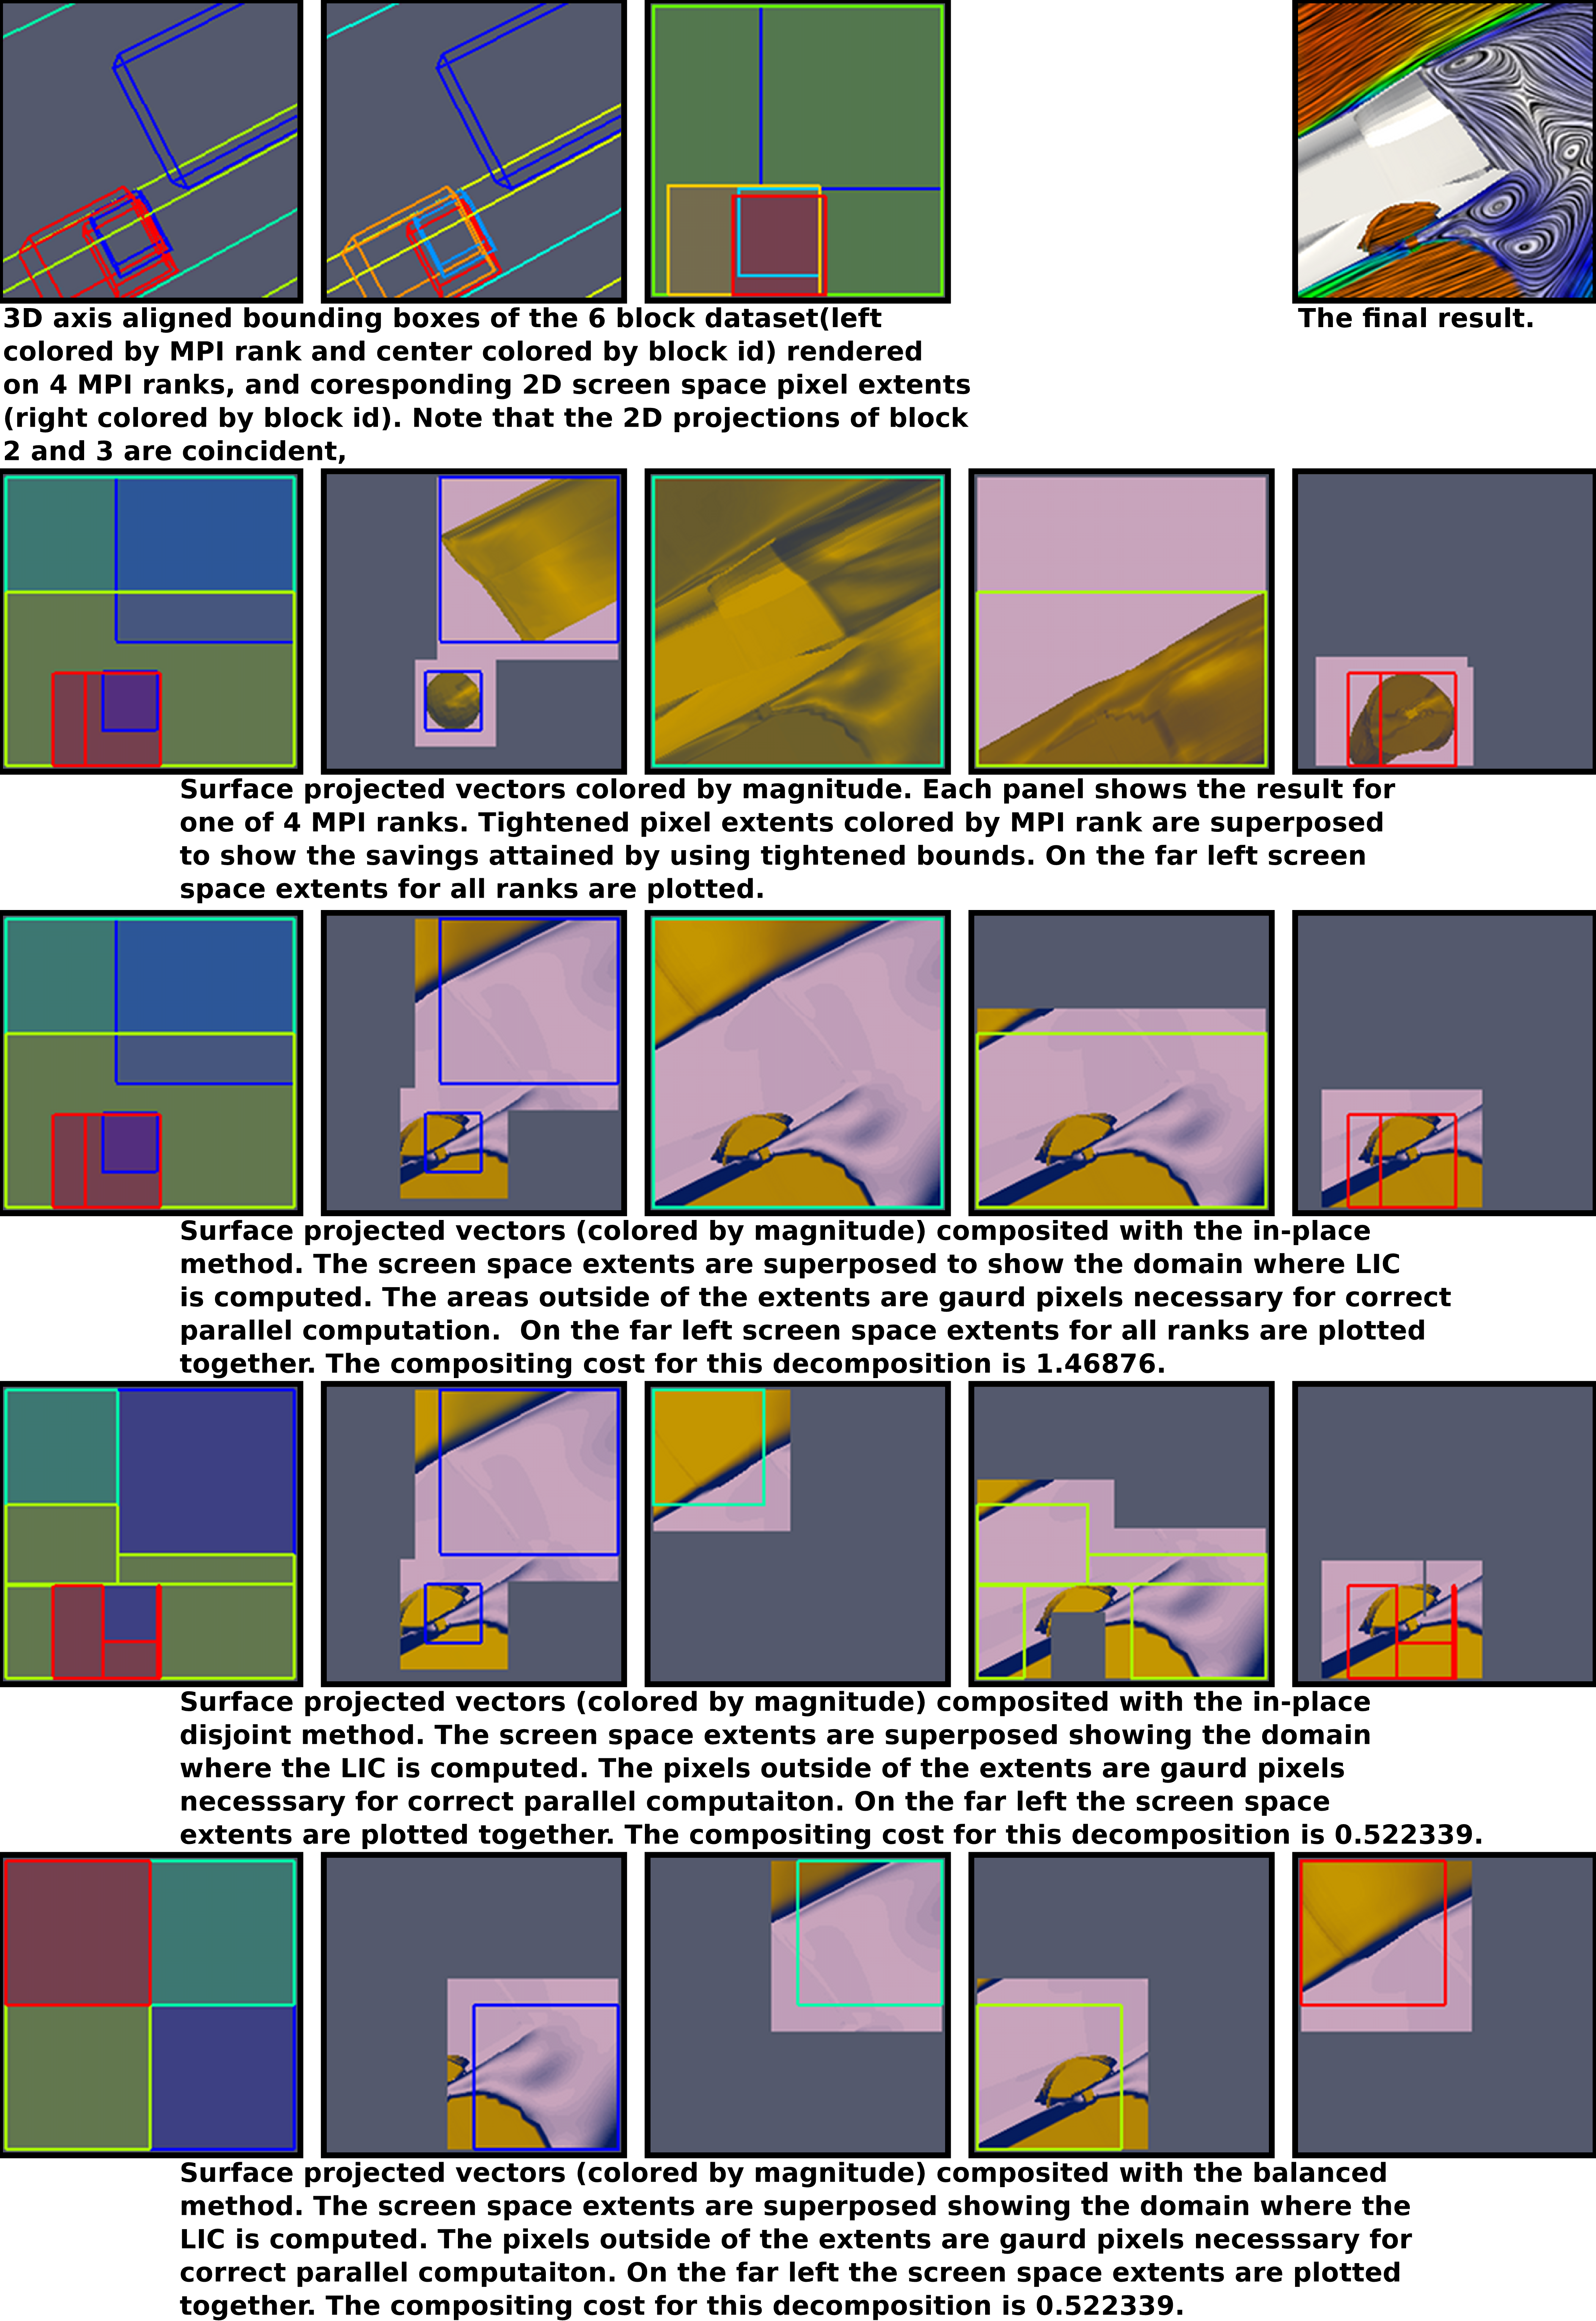
\includegraphics[width=0.9\textwidth]{./images-data/compositing-200ppi.png}
 % compositing-200ppi.png: 4269x6208 pixel, 200dpi, 54.22x78.84 cm, bb=0 0 1537 2235
 \caption{Compositing algorithms}
 \label{fig:compositing}
\end{figure}

\FloatBarrier






\subsection{Compositor Scaling}
Over the past few days I've been analyzing the new parallel surface lic algorithms scalability and performance and I thought you might find the early results helpful as you look at the code. These runs were made with pvpython+pvserver on NERSC's Cray XC30 Edison using Mesa 9.2.0's OS Mesa llvmpipe driver with 4 rendering threads per rank and 8 ranks per node. There's also some documentation of the compositors in this talk (see the last few slides) http://www.hpcvis.com/vis/talks/rdav-ah-2013/rdav-ah-2013.pdf

\begin{figure}[h]
 \centering
 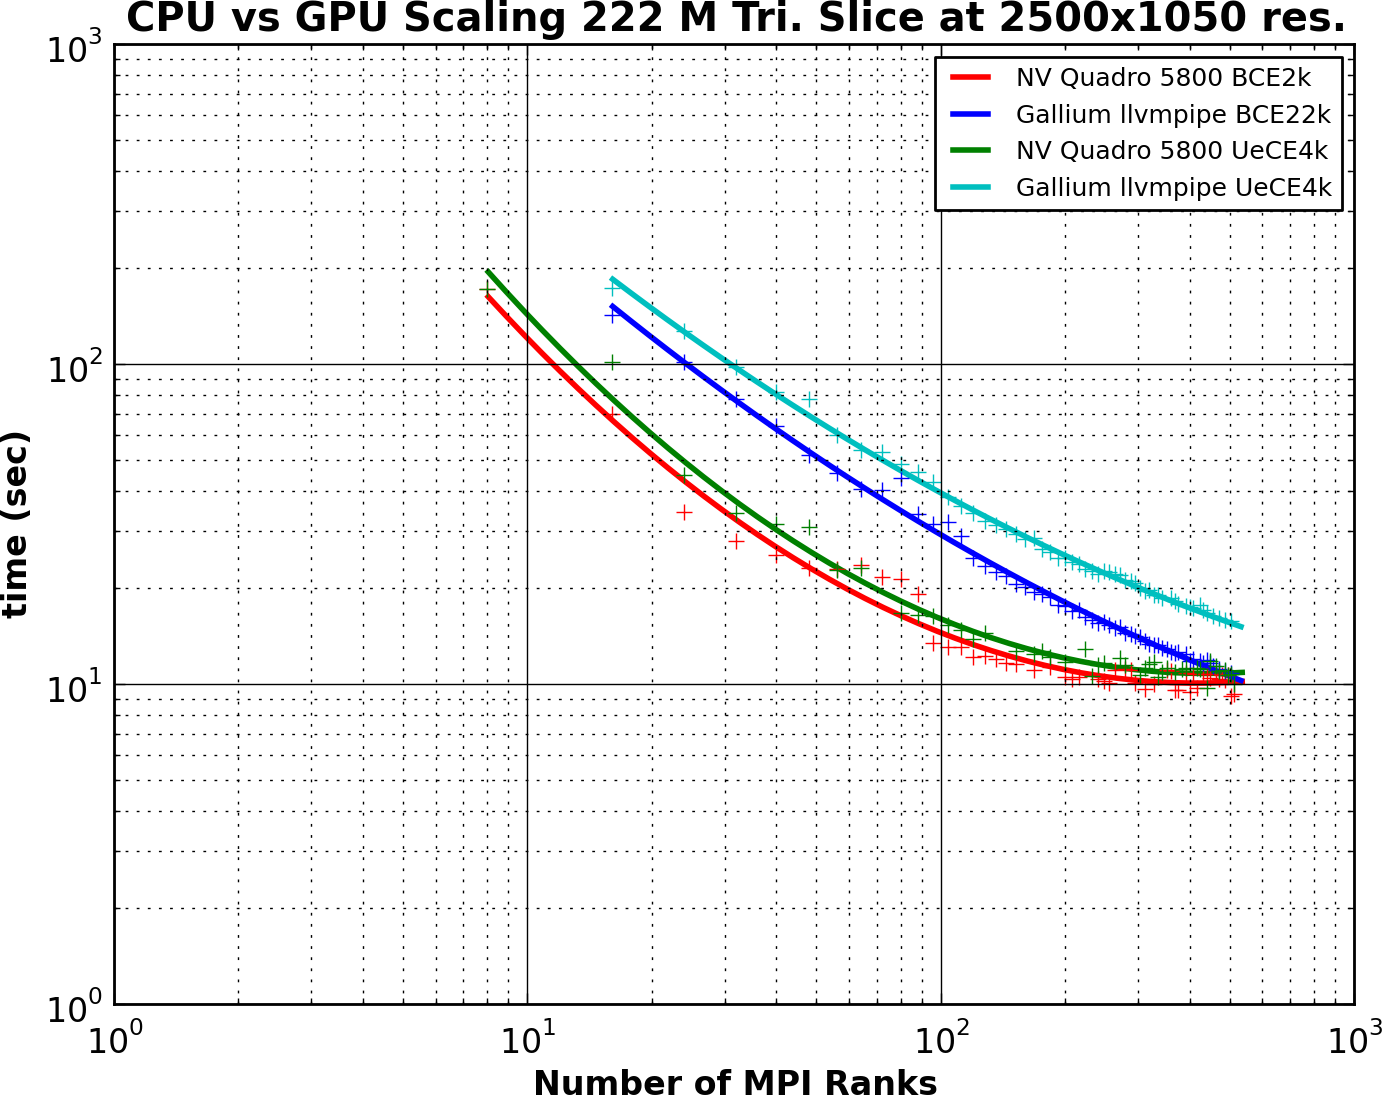
\includegraphics[width=0.8\textwidth]{./scaling-ce-slice-gpu.png}
 % scaling-ce-slice-gpu.png: 1600x1200 pixel, 200dpi, 20.32x15.24 cm, bb=0 0 576 432
 \caption{Test of CE scaling on two vector fields}
 \label{fig:ce-scaling}
\end{figure}
This figure shows scaling from 16 to 512 ranks on a massive 16384x8192 VPIC dataset.  The figure shows runs on two vector fields using the settings for a high quality image with and without the new contrast enhancement feature. The figure shows that although the new CE feature makes use of MPI\_Allreduce this does not negatively impact scaling. The differences in performance are attributable to the difference in number of integration steps. Typically I've found that to get the look I want I end up using more integration steps when CE is enabled. A sample image from this run is here: http://www.hpcvis.com/vis/vtk-surface-lic-parallelization/kh-new-jaguar-lic-b-woce.png


\begin{figure}[h]
 \centering
 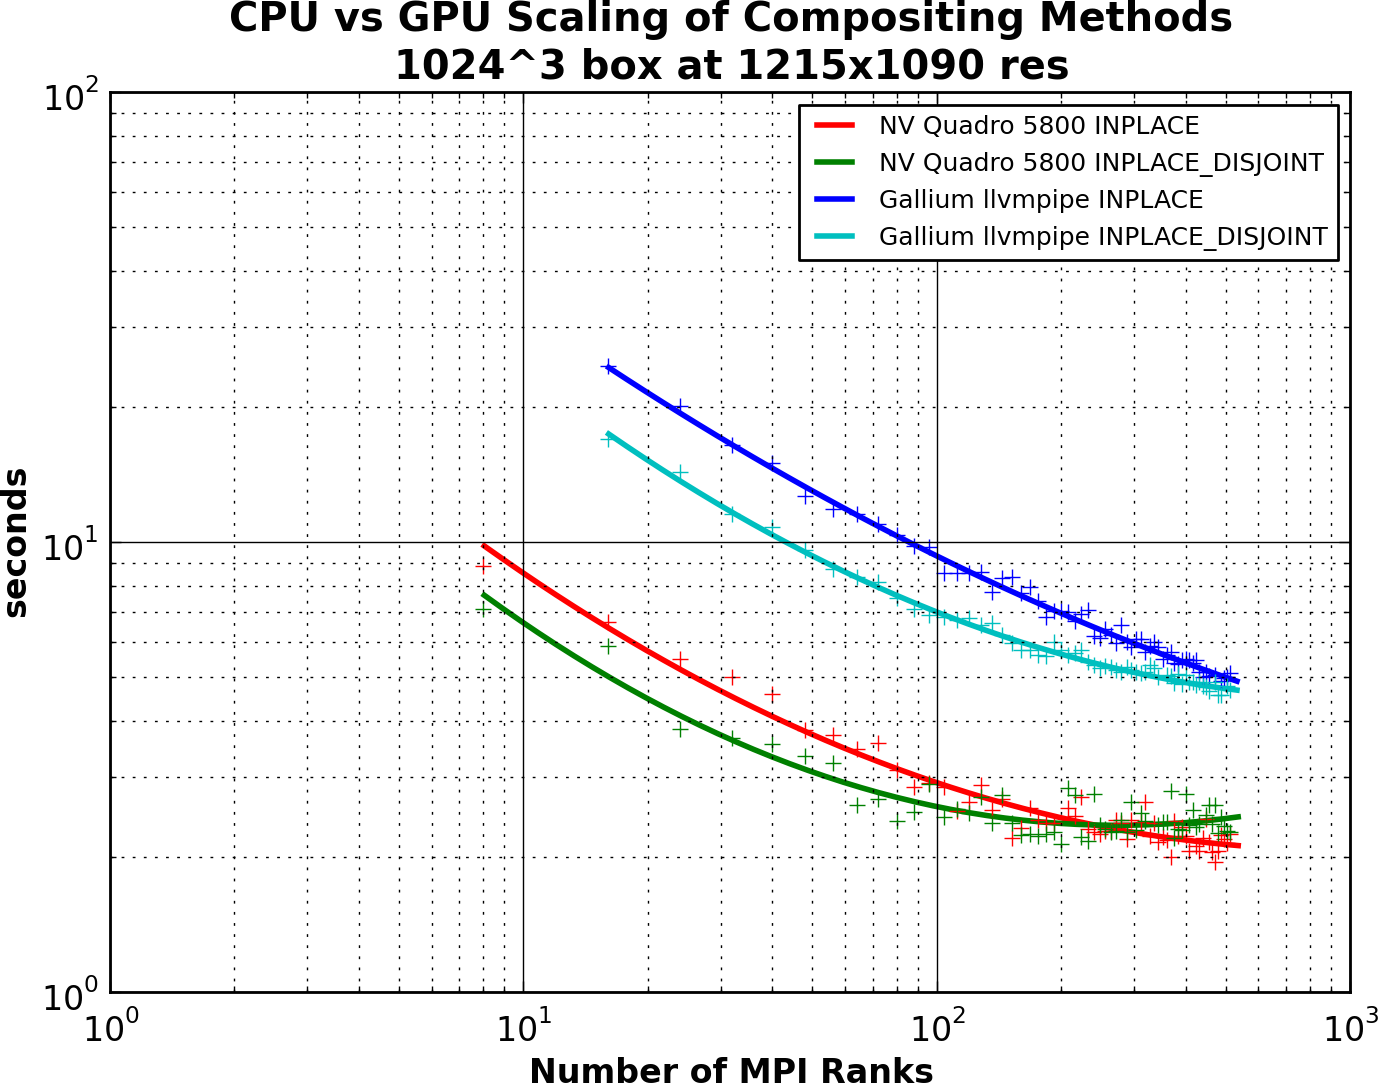
\includegraphics[width=0.8\textwidth]{./scaling-composite-cube-gpu.png}
 % scaling-composite-cube-gpu.png: 1600x1200 pixel, 200dpi, 20.32x15.24 cm, bb=0 0 576 432
 \caption{Compositor scaling on MHD turbulence dataset}
 \label{fig:comp-scaling}
\end{figure}
This figure show scaling from 16 to 512 ranks on a large $1204^3$ MHD turbulence dataset and a comparison of two of the compositing algorithms. The INPLACE option is what you and I had initially discussed on Skype, while the INPLACE\_DISJOINT option ensures that each fragment is computed only once by uniquely assigning ownership of regions of the screen to ranks while leaving the data in-place ie. a rank doesn't take ownership of a fragments it doesn't have data for. For the INPLACE\_DISJOINT approach the compositing communication cost is the same or in some cases less than the INPLACE approach although it's split into two phases(gather and scatter). The figure shows that the INPLACE\_DISJOINT method offers a nice increase in performance. The speed up is larger in the smaller runs because in those runs the screen regions by rank are larger, and this presents a greater opportunity to reduce the number of fragments processed per rank. The following teo plots show this better. The image produced by these runs is here: http://www.hpcvis.com/vis/vtk-surface-lic-parallelization/pr1-lic.png

\begin{figure}[h]
 \centering
 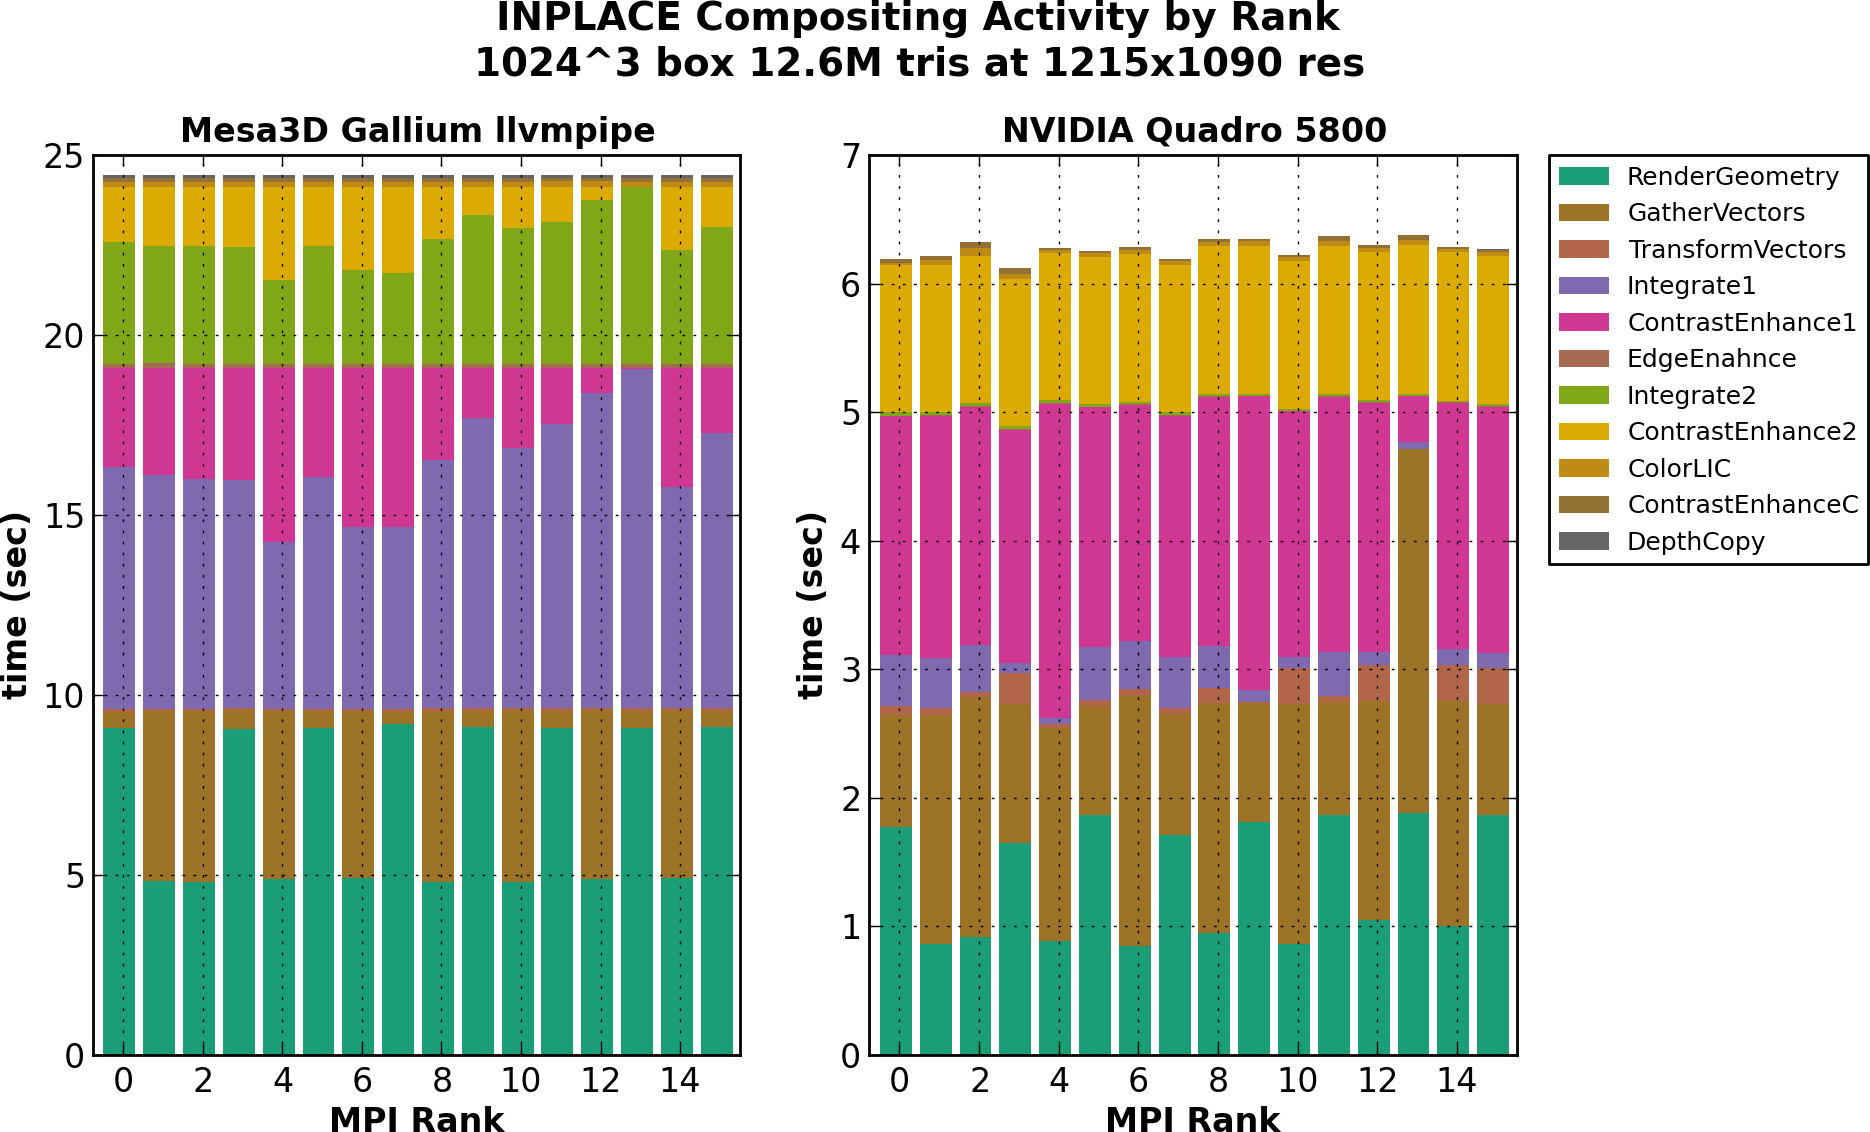
\includegraphics[width=1.1\textwidth]{./scaling-gant-inplace-composite-gpu-mesa.png}
 % scaling-gant-inplace-composite-gpu-mesa.png: 2046x1095 pixel, 200dpi, 25.98x13.91 cm, bb=0 0 737 394
 \caption{INPLACE Compositing}
 \label{fig:inplace-comp}
\end{figure}


These two figures are Gant plots of each rank's activity during the 2 node 16 rank compositing INPLACE and INPLACE\_DISJOINT scaling runs. We're looking at the 2-node case because it shows the greatest speed up for the INPLACE\_DISJOINT compositor and it will be easier to see the performance differences between the two. For both runs most of the time is spent in RenderGeometry (vector projection and light vertex shaders) and Integrate1/Integrate2 phases. CE phases tend to look long because of the MPI\_Allreduce ranks get synchronized by the slowest rank so most of the time spent there is waiting. The RenderGeometry and GatherVectors(compositing and guard pixel exchange) times are nearly identical for both compositors. This means that speed up attained by the INPLACE\_DISJOINT compositor is a result of reduced integration time while computing the LIC. With INPLACE\_DISJOINT approach each rank has fewer fragments to process and there's a greater opportunity to cull empty fragments as the screen space regions are decomposed. These plots also show that the overhead of decomposing(makiing the screenspace disjoint amongst ranks) is small enough to be negligible and that although the INPLACE\_DISJOINT moves less data around during compositing and guard pixel exchange it doesn't contribute a lot to the speed of the approach.

\begin{figure}[h]
 \centering
 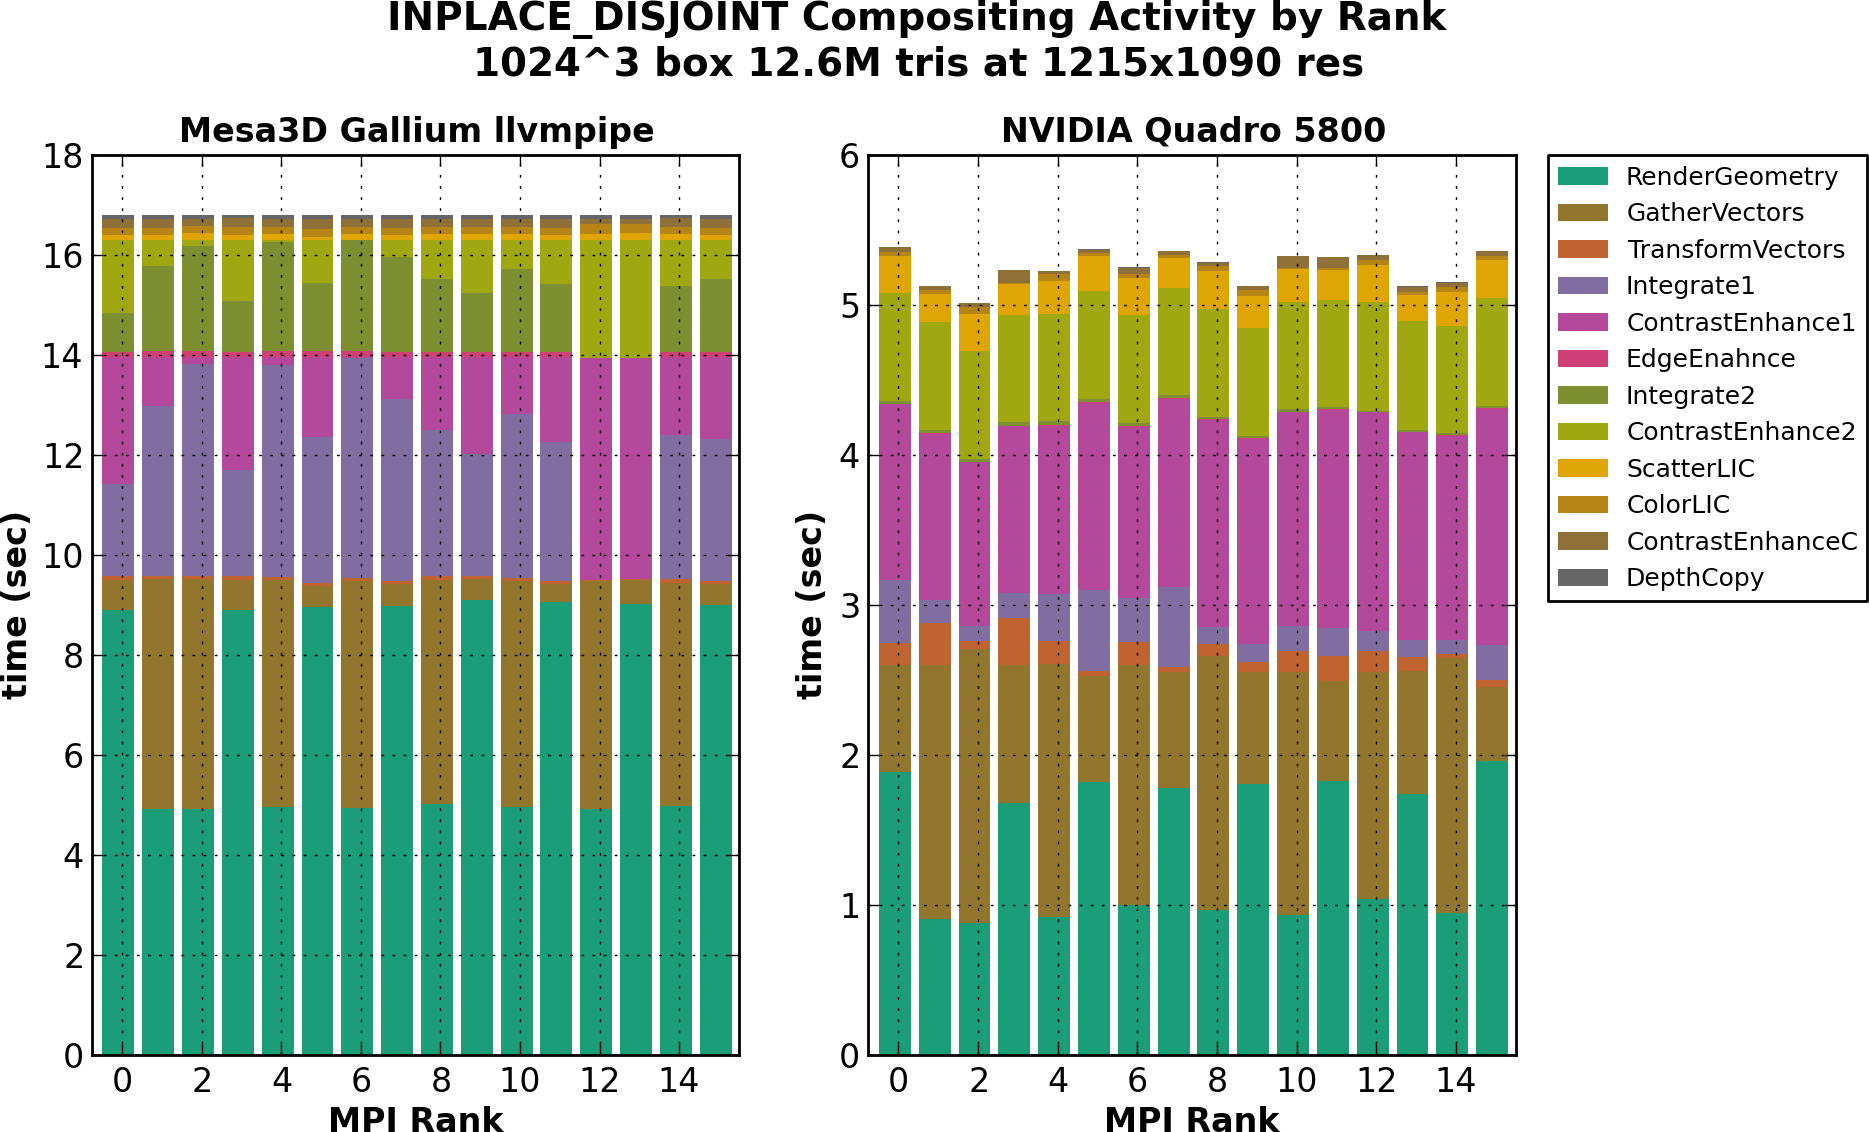
\includegraphics[width=1.1\textwidth]{./scaling-gant-inplace-disjoint-composite-gpu-mesa.png}
 % scaling-gant-inplace-disjoint-composite-gpu-mesa.png: 2128x1096 pixel, 200dpi, 27.03x13.92 cm, bb=0 0 766 395
 \caption{DISJOINT Compositor}
 \label{fig:disj-comp}
\end{figure}



\end{document}